\section{Rischio biologico delle professioni sanitarie}

\subsection{Virus dell'epatite B}

\subsubsection{Epidemiologia}

  Sono documentati oltre 2 miliardi di soggetti al mondo che si sono
  infettati in qualche momento della loro vita

  4 milioni di nuovi casi di epatite acuta ogni anno nel mondo

  240 milioni di portatori sani

  >780.000 soggetti muoiono ogni anno per patologie
  correlate ad HBV: cirrosi epatica e il carcinoma epatocellulare

  Per quanto riguarda la prevalenza di infezione cronica da HBV
  distinugiamo zone:

\begin{itemize}
\item
  \emph{Alta prevalenza} (>8\% della pop che presenta
  HBsAg): 45\% della popolazione mondiale, rischio durante la vita
  >60\% di infettarsi

  Infezione nella prima infanzia molto frequente
\item
  \emph{Prevalenza intermedia} (italia) (2-7\% della pop con HBs Ag):3\%
  della popolazione mondiale,

  rischio durante la vita 20-60\% di infettarsi

  Infezione può avvenire in tutti i gruppi di età
\item
  \emph{Bassa prevalenza} (<2\% della pop che presenza HBsAg):
  12\% della popolazione mondiale, rischio durante la vita
  >20\% di infettarsi
\end{itemize}
  Infezione colpisce gruppi di adulti a rischio

  \emph{\emph{In italia:}}

  I portatori cronici (prevalenza 1,5\%) sono 600.000: questo è molto
  importate in termini sanitari e anche per sanità pubblica perche ogni
  soggetto che alberga il virus è un soggetto trasmettitore quindi una
  potenziale sorgente di infezione

  Incidenza 1/100.000 abitanti/anno

  Cirrosi 100.000

  Morti/anno 1.500 per patologie correlate

\subsubsection{Aspetti micorbiologici}

  \emph{\emph{Famiglia:}}Virus facente parte della famiglia degli
  Hepadnaviridae

  Nel sangue dei soggetti infetti si riscontrano 3 tipologie di
  particelle al microscopio elettronico:

\begin{itemize}
\item
  particella di Dane: che è il virus completo, di dimensioni di 42 nm,
  dotata di acido nucleico e strutture di superficie
\item
  strutture tubulari: che costituiscono materiale antigenico in eccesso,
  prive di acido nucleico quindi non infettanti e significative solo dal
  punto di vista antigenico
\item
  particelle rotonde piccole
\end{itemize}
  \emph{\emph{Genoma}}: virus a DNA cricolare incompleto (parzialmente
  bicatenario) con DNA polimerasi virus codificata, sono stati
  riconosciti 6 genotipi che però non inficiano l'attività del vaccino.
  E' un virus che è in grado di intergarsi al DNA dell'epatocita.

  Sono stati identificati 4 geni:

\begin{itemize}
\item
  Gene C che codifica per proteine del CORE
\item
  Gene P che codifica per DNA-polimerasi DNA dipendente
\item
  Gene S che codifica per le proteine del pericapside
\item
  Gene X che codifica per le chinasi
\end{itemize}
  Sono stati identificati 3 antigeni:

\begin{itemize}
\item
  \textbf{HbsAg}: (antigene strutturale) antigene di superficie,
  rappresenta le proteine del pericapside delle particelle di Dane ma
  anche delle particelle vuote. E' costituito da due gruppi di
  determinanti mutuamente esclusivi che si combinano variamente nelle
  varie regioni del pianeta. E' la struttura necessaria alla
  penetrazione del virus nella cellula.
\item
  \textbf{HbeAg}: (antigene non strutturale) è un antigene di funzione
  che è presente nella fase attiva del virus
\item
  \textbf{HbcAg}: (antigene strutturale) proteine del core
\end{itemize}
  Sono tutti e tre immunogeni ma l'unico che ci interessa dal punto di
  vista della protezione è HbsAg che porta alla produzione di anticorpi
  neutralizzanti (anti-HBsAg) che impediscono la penetrazione del virus
  nella cellula.

\subsubsection{Storia naturale dell'infezione} a seguito dell'infezione abbiamo un periodo di
  incubazione di 30-80 giorni, e dopo possiamo avere:

\begin{itemize}
\item
  nel 90-95\% dei casi: infezione asintomatica,
\item
  nel 5-10\% dei casi: infezione clinicamente evidente, di cui l' 1\%
  dei casi è un'epatite fulminante
\end{itemize}
  da entrambi i casi può derivare una cronicizzazione, nel 10\% dei casi
  totali, a cui poi seguono i danni da cronicizzazione che sono: cirrosi
  ed epatocarcinoma.

  La risoluzione negli adulti è molto frequente (>90\%)

\subsubsection{Clinica} 
Clinicamente, se
  l'infezione è clinicamente evidente, abbiamo 3 fasi:

\begin{itemize}
\item
  fase prodromica: malessere, nausea, vomito, affaticamento, anoressia,
  mialgie e febbricola
\item
  fase itterica: comparsa di urine bruno-dorate, feci acoliche, ittero,
  epatosplenomegalia
\item
  fase di convalescenza: normalizzazione di enzimi epatici
\end{itemize}
  Nel bambino è tendenzialmente asintomatica, mentre con il crescere
  dell'età aumentano le manifestazioni cliniche.

  La tendenza alla cronicizzazione invece è al contrario: il bambino
  alla nascita e nel primo anno di vita ha un rischio di cronicizazzione
  del 90\%; più l'infezione è precoce, più è il rischio di cronicizzare.

\subsubsection{Patogenesi} 
è un virus che
  replica all'interno delle cellule in cui è in grado di penetrare
  tramite l'HbsAg con cui si aggancia principalmente alla cellula
  epatica, ma anche a monociti, linfociti, fibroblasti. Il danno al
  fegato è un danno indiretto non citocida.

\subsubsection{Studio degli Ag} 
Lo studio
  degli antigeni nel sangue ci consente di fare diagnosi e di stadiare
  le varie fasi della malattia:

\begin{figure}[!ht]
\centering
	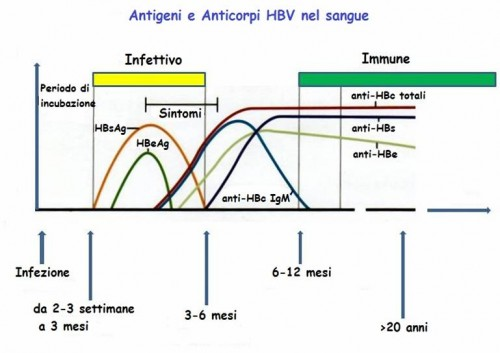
\includegraphics[width=0.3\textwidth]{11/image1.jpeg}
	\end{figure}

  \emph{In questa immagine vediamo la fase di infezione della malattia a
  cui segue la fase di risoluzione:}

  Dopo 4 settimane abbiamo la comparsa dell'HBsAg.

  Poco tempo dopo, quasi contemporaneamente abbiamo la comparsa di HBeAg
  (antigene di funzione che indica l'attività di replicazione del virus)
  e quando raggiunge il suo apice di concentrazione abbiamo
  l'espressione clinica della malattia.

  Alla comparsa di HBeAg segue la comparsa degli anticorpi: anti- HBc
  che prima sono di classi IgM, a breve durata di qualche mese, e poi
  IgG che permangono per tutta la vita.

  Nell'immagine vediamo un quadro di risoluzione per cui HBsAg si
  estingue attorno alla 24esima settimana ma passano molte settimane
  prima che compaiano gli anticorpi, quindi non abbiamo MAI
  sovrapposizione tra HbsAg e Anti-HBs (!!), sono mutuamente esclusivi e
  infatti nella diagnostica non bisognerà mai cercarli
  contemporanemente.

  Anche HBeAg è in grado di fare produrre anticorpi ma né Anti-HBe né
  Anti-HBc sono protettivi, li sfruttiamo solo dal punto di vista
  diagnostico per comprendere la fase in cui ci troviamo.

  Nella fase di non evidenziazione del HBsAg e prima che compaiano gli
  Anti-HBs abbiamo un \textbf{periodo finestra}, buio dal punto di vista
  diagnostico in cui abbiamo solo gli anti-HBc (non troviamo mai HBcAg
  nel sangue libero, lo troviamo solo dentro gli epatociti quindi per
  identificarlo è necessario fare delle biopsie). In questa condizione
  il soggetto sta ancora combattendo contro il virus quindi nella
  maggior parte dei casi è ancora infettante.

\begin{figure}[!ht]
\centering
	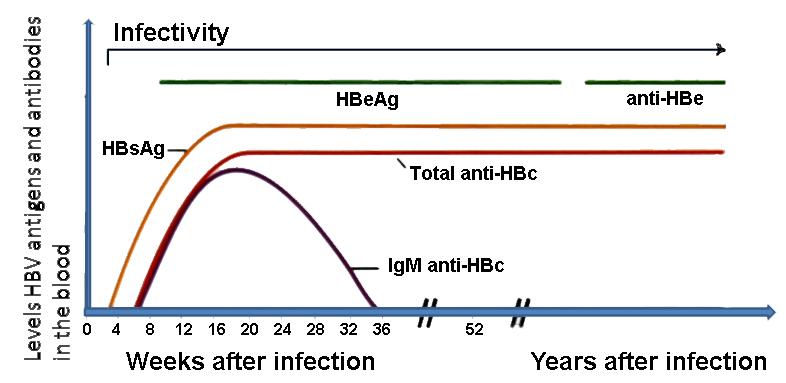
\includegraphics[width=0.3\textwidth]{11/image2.png}
	\end{figure}

  \emph{In questa immagine vediamo invece l'evuoluzione sierologica
  verso un quadro di cronicizzazione:} HBsAg non scompare mai e anche
  anti-HBc continua ad essere prensente (prova che anti-HBc non hanno
  significato protettivo), abbiamo la presenza per lungo tempo di HBeAg
  infatti è un virus che si replica, e mancano completamente gli
  anti-HBs.

\begin{figure}[!ht]
\centering
	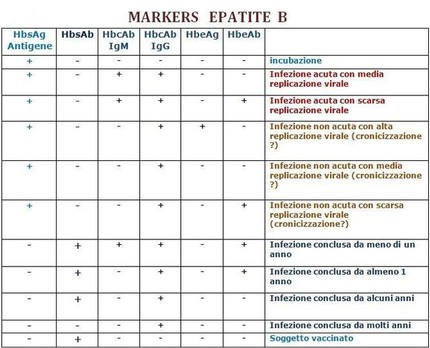
\includegraphics[width=0.3\textwidth]{11/image3.jpeg}
	\end{figure}

\subsubsection{Diagnosi}

  Dobbiamo interpretrare i markers dell'epatite B che sono numerosi, da
  un lato abbiamo gli antigeni e dall'altro gli anticorpi e questi
  possono essere presenti in diverse combinazioni:

\begin{itemize}
\item
  tutto negativo: il soggetto è sucettibile.
\item
  HbsAg negativo, Anti-HBc positivo, Anti-HBs positivo: soggetto immune
  per infezione naturale, quindi ha avuto e superato la malattia.
\item
  HBsAg negativo, Anti-HBc negativo,Anti-HBs positivo: soggetto
  vaccinato, infatti è venuto in contatto solo con HbsAg. Immune per
  vaccinazione
\item
  HBsAg positivo,Anti-HBc positivo, IgM anti-HBc positivo,Anti-HBs
  negativo: soggetto con infezione acuta in atto.
\item
  HBsAg positivo, Anti HBc positivo, IgM anti-HBc negativo, Anti-HBs
  negativo: soggetto con infezione cronica
\item
  HBsAg negativo,Anti HBc positivo, Anti-HBs negativo: quattro ipotesi ->
  soggetto immune in cui sono scomparsi gli anticorpi Anti-HBsAg che ha
  avuto la malattia tantissimo tempo fa; soggetto in cui gli Anti-HBsAg
  sono ancora troppo bassi; errore del test; soggetto in fase finestra.
\end{itemize}

\subsubsection{Trasmissione} 
Può essere trasmesso
  tramite liquidi biologici che possono essere suddivisi in base alla
  concentrazione di HBV in tre gruppi:

\begin{itemize}
\item
  Bassa concentrazione: urine, feci, latte, lacrime, sudore; sono
  trascurabili perché non hanno peso epidemiologico
\item
  Media concentrazione: saliva, liquidi seminale, secrezioni vaginali
\item
  Alta concentrazione: sangue, siero, essudati
\end{itemize}
 
  Le modalità classiche di trasmissione sono:

\begin{itemize}
\item
  Parenterale:
\begin{itemize}
\item
  \emph{Apparente}: atti chirurgici, ferite, emotrasfusione (anche se
  in Italia questo problema non è mai stato elevato, infatti le
  donazioni sono libere), scambio di siringhe, punture accidentali con
  aghi, sterilizzazione inadeguata (trascurabile ma da non dimenticare),
  body art..
\item
  \emph{Inapparente}: strumenti di uso comune come spazzolini,
  asciugamani e pettini sono degli strumenti che possono esporre a
  rischio i soggetti suscettibili. Sono le principali cause di HBV ad
  eziologia non nota perché è difficile ricordarsi di avere avuto queste
  esposizioni.
  \end{itemize}
\item
  Verticale: transplacentare e la perinatale (quella che prevale). Nella
  trasmissione perinatale il neonato ha un rischio minimo del 70\% di
  infettarsi se la madre presenta una doppia antigenemia e del 60\% se
  la madre è solo HBsAg positiva, e quindi quelli infetti nel 90\% dei
  casi evolveranno in cronicizzazione.
\item
  Sessuale (quasi il 50\%)
\end{itemize}
  La sorgente di infezione è l'uomo, è una malattia specie specifica.
  L'uomo è infettante durante il periodo di incubazione (diverse
  settimane prima della comparsa dei sintomi), durante il periodo di
  convalescenza (due mesi dopo la scomparsa dei sintomi) e nella fase
  cronica della malattia. Quindi abbiamo come sorgenti di infezione: il
  soggetto malato, il portatore precoce, il portatore cronico e il
  portatore convalescente.

  L'infettitività è tanto maggiore quanto più è presente l'HBsAg, e la
  doppia antigenemia (HbeAg) depone per un'elevata carica infettante.

\paragraph{Soggetti a rischio}

  I soggetti a rischio di infezione sono:

\begin{itemize}
\item
  bambini che nascono da madre infetta
\item
  tossico dipendenti che usano droghe endovena
\item
  emodializzati
\item
  operatori sanitari: nell'ambito degli operatori sanitari ci sono
  categorie più a rischio: chirurghi, patologi anatomo patologhi,
  odontoiatri, tecnici di laboratorio, infermieri..
\item
  omosessuali maschi
\item
  partner di soggetti HBsAg positivi,
\item
  soggetti che usano body art
\item
  detenuti.
\end{itemize}

\subsubsection{Prevenzione}

  E' una malattia soggetta a notifica obbligatoria, malattia di classe
  2, è molto importante l'accertamento diagnostico, e l'inchiesta
  epidemiologica che si avvale dei test diagnostici per capire se
  abbiamo dei soggetti suscettibili o dei soggetti portatori in modo da
  istruire i soggetti: il soggetto suscettibile sarà invitato a fare il
  vaccino, il soggetto portatore sarà istruito alle norme igieniche da
  adottare e con lui anche i suoi conviventi.

  Lo sviluppo della prevenzione è iniziato negli anni '70 con la
  scoperta di metodiche di rilevazione dei marker di infezione che hanno
  permesso di definire le modalità di trasmissione del virus e le più
  importanti pratiche a rischio.

  Negli anni '80 si ebbe la scoperta dei primi efficaci vaccini che ha
  permesso di attuare un'immunoprofilassi attiva in soggetti a rischio e
  quindi di ridurre le sorgenti di infezione.

  Processo di disinfezione e sterilizzazione: autoclave, ipoclorito,
  composti fenolici e glutaraldeide. E' un virus che ha un'elevata
  resistenza nell'ambiente, è stato trovato anche ne sangue essiccato
  dopo un mese.

\paragraph{Profilassi}

  Disponiamo di una profilassi attiva e passiva:

\begin{itemize}
\item
  \textbf{Immunoprofilassi passiva} è costituita da Ig specifiche
  preformate, la sua efficacia dipende dal numero di dosi (Ig hanno una
  vita di circa un mese, se il virus permane per oltre un mese il
  soggetto è scoperto) e dalla precocità del trattamento.

  E' indicato in adulti post esposizione come ad esempio: contatto con
  liquidi infetti sulle mucose, puntura accidentale, contagio per
  trasmissione sessuale. In questi casi si deve fare sia l'applicazione
  della profilassi passiva e in contemporanea dell'attiva.
\item
  \textbf{Immunoprofilassi attiva} costituita dal vaccino: la prima
  preparazione del vaccino fu preparata a partire da sangue di soggetti
  infetti usando esclusivamente l'HBsAg, questo vaccino era estremamente
  costoso e raro per via del problema della sicurezza (richiedeva molti
  passaggi).
\end{itemize}
  Negli anni '90, usando le tecniche del DNA ricombinante si è potuto
  produrre a costi inferiori il vaccino e questo ha consentito di
  imporre la vaccinazione ai nuovi nati dal 1991. Quindi il vaccino in
  uso è un vaccino ricmbinante con un'efficacia del 95\%, con
  oscillazioni che sono legate alla persona (stato di salute, età..), la
  scheda di somministazione è composta da 3 dosi e non è prevista una
  dose booster (aggiunitiva) nella popolazione generale ma solo in
  specifici gruppi.

  La capacità immunogena dipende da variabili come età, sesso, stato
  immunitario, patologie concomitanti e dalla schedula vaccinale, quindi
  il risultato della vaccinazione può essere:
\begin{itemize}
\item soggetti non responder: non rispondono allo stimolo antigenico
\item soggetti responder : possono rispondere in modo più o meno
  ottimale. È una delle poche vaccinazioni che ha un correlato
  immunologico: abbiamo un valore al di sotto del quale non abbiamo
  protezione immunologica e al di sopra del quale abbiamo la protezione.
  In base al valore distinguiamo 3 gruppi:

\begin{itemize}
\item
  IPO (<10mUl/mL) che sono sotto il valore di protezione;
\item
  LOW (10-100mUl/mL);
\item
  GOOD (>100mUI/mL).
\end{itemize}
\end{itemize}
  Nel tempo abbiamo una riduzione degli anticorpi, il grosso della
  riduzione avviene nei primi 5 anni e dopo il valore degli ab risulta
  essere stabile, quindi è importante il livello di partenza.

  Quindi la necessità di una doser booster è riservata a quei soggetti
  che sono IPO, e dopo la somministrazione della dose booster si arriva
  sempre al valore necessario di ab. Ma non tutti i soggetti IPO devono
  fare la dose booster ma solo i soggetti fortemente a rischio come: il
  personale sanitario, detenuti, zone di alta endemia, soggetti che
  usano droghe, soggetti HIV positivi.. la popolazione generale non deve
  fare una rivaccinazione ( nel caso in cui contraessero l'infezione è
  come se facessero una dose booster).

  Effetti avversi: La somministrazione del vaccino può dare degli
  effetti collaterali locali, tra cui dolore e arrossamento ma comunque
  trascurabili e transitori, ed effetti collaterali generali, molto
  rari, come cefalea e febbricola transitori. Eventualità di anafilassi
  è 1/600.000, non ci sono studi che correlino il vaccino con SM o con
  Guillain Barrè.

  E' un vaccino ampiamente disponibile, relativamente poco costoso e
  sicuro.

  In Italia dal 1991 il vaccino è somministrato gratuitamente e
  obbligatoriamente a tutti i nuovi nati dal 3 mese di vita e per tutti
  quei soggetti che compivano 12 anni. In questo modo dal 2003 (fine
  della vaccinazione dei 12enni) tutti i soggetti fino ai 24 anni
  risultano immuni al virus, ora è stata superata ampiamente la fascia
  dei 30 anni.

\begin{figure}[!ht]
\centering
	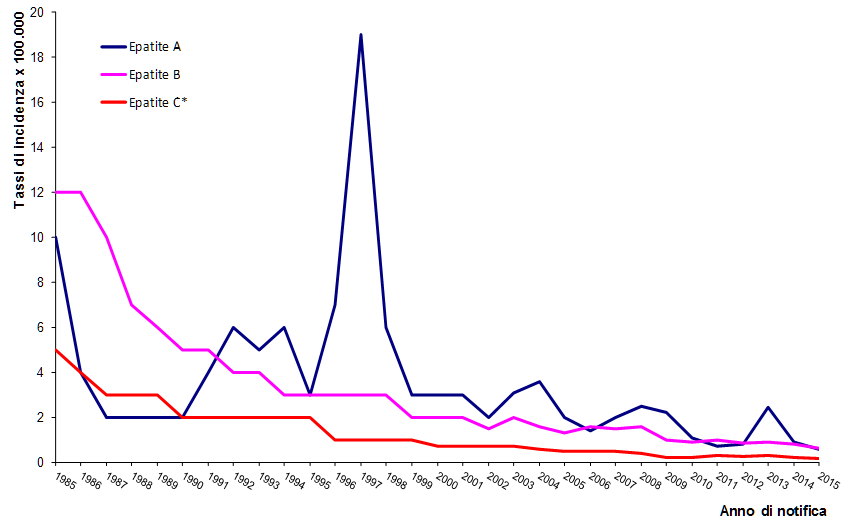
\includegraphics[width=0.3\textwidth]{11/image4.png}
	\end{figure}

  Con il vaccino abbiamo avuto un significativo calo di incidenza dalla
  malattia che era era già iniziato prima grazie all'applicazione,
  secondo legge, di norme di comportamento e norme di precauzione
  standard /generale.

  Le \emph{norme di precauzione generale} nascono dal concetto che tutti
  i liquidi biologici (sangue, siero, sperma..) e materiali biologici
  contaminati da sangue devono essere considerati infetti, ma non solo
  quelli di soggetti infetti ma anche quelli di qualsiasi persona devono
  essere considerati come potenzialmente infetti. Sono quindi delle
  procedure che sono da applicare a tutti i soggetti.

  Le \emph{norme di legge} sono: notifica obbligatoria, con tutte le
  inchieste tra cui l'inchiesta epidemiologica; controllo di tutte le
  unità di sangue (emotrasfusioni, emoderivati..); vaccinazione
  obbligatoria dal 1991 per tutti e in particolare per personale
  sanitario; offerta gratuita del vaccino per persone a rischio.

\subsection{Virus dell'epatite delta}

  E' un virus difettivo, non è in grado di infettare autonomamente le
  cellule ma lo fa solo se può rivestirsi dell'HBsAg, quindi l'infezione
  avviene solo in concomitanza con infezione con HBV.

  Le condizioni in cui si può sviluppare sono quindi condizionate dallo
  stato immunitario del soggetto nei confronti del virus dell'epatite B:
  quindi

\begin{itemize}
\item
  \emph{Se un soggetto è suscettibile} potrebbe COINFETTARSI con HBV e
  HDV, e nel caso entrasse in contatto solo con HDV non succederebbe
  nulla.
\item
  \emph{Se un soggetto è immune} ad HVB non potrà mai infettarsi con HDV
\item
  \emph{Se un soggetto è infetto} con HBV e quindi con HBsAg
  disponibile, potrebbe SOVRAINFETTARSI con HDV.
\end{itemize}

\subsubsection{Trasmissione}
 parenterale,
  verticale e sessuale

\subsubsection{Epidemiologia} sottostimata,
  raramente si cercano i marcatori per il delta

\subsubsection{Clinica}

  L'infezione è sintomatica con un decorso clinico più grave
  dell'epatite B e con un aumentato rischio di epatite fulminante.
  Coinfezione e sovrainfezione hanno un quadro clinico differente:

\begin{itemize}
\item
  La coinfezione si manifesta come un quadro di epatite, e non aumenta
  il rischio di cronicizzazione
\item
  La sovrainfezione ha un quadro decisamente più grave con innalzamento
  degli enzimi epatici anche per tempi più prolungati, aumenta il
  rischio di cronicizzazione e aumenta anche il danno epatico
  \end{itemize}

\subsubsection{Prevenzione}

  Differente a seconda se il soggetto è gia infetto o meno da HBV:

\begin{itemize}
\item
  se è una coinfezione si deve fare una profilassi pre e post infezione
  del HBV, perché, indirettamente, ostacolando HBV si impedisce la
  formazione di HBsAg e quindi la replicazione di HDV.
\item
  Nel caso del rischio di una sovrainfezione dobbiamo informare il
  soggetto del rischio e di tutte le norme che devono essere applicate.
\end{itemize}

\subsection{Virus dell'epatite C}

\subsubsection{Epidemiologia}

  4 milioni di nuovi caso anno

  Morti 500.000 anno

  Prima causa di trapianto di fegato

  A livello mondiale di sono 140 milioni di persone infette, che sono
  variamente distribuite: al primo posto Africa, seguita da Mediterraneo
  orientale, seguito da Pacifico occidentale; l'Europa ha una sua
  importanza ma decisamente minoritaria rispetto alle altre.

\subsubsection{Aspetti microbiologici}

  \emph{\emph{Famiglia:}} Flaviviridae.

  \emph{\emph{Envelope}} lipidico (magiore fragilità per disinfettanti).

  \emph{\emph{Genoma:}} Virus ad RNA. Ci sono tantissimi genotipi, con
  alta variabilità in particolare nelle zone NS (non strutturali). Da 1
  a 6 sono i genotipi principali, da cui poi derivano i sotto genotipi
  che sono più di 100. Ci sono molti studi che correlano il genotipo con
  il decorso della malattia e la risposta ai farmaci.

\subsubsection{Clinica}

\begin{itemize}
\item
  la maggior parte delle forme sono silenti,
\item
  la forma clinicamente evidente la abbiamo nel 5\%,
\end{itemize}
  Su tutti gli infetti grava una possibilità di cronicizzazione
  elevatissima del 85\%, e su questi cronici il 20\% può degenerare in
  cirrosi e separatamente in epatocarcinoma.

  Importante è ricordare le cause di cirrosi: l'alcool è causa di
  cirrosi nel 30\%, mentre un ruolo decisamente più importante è
  rivestito dalle infezioni virali epatiche che sono causa del 50\% dei
  casi di cirrosi (HBV nel 12\% dei casi; HCV 36\% dei casi).

  Fattori che possono favorire lo sviluppo della malattia sono:

\begin{itemize}
\item
  alcol
\item
  età: una prima infezione in eta>40 anni predispone alla
  cronicizzazione
\item
  coinfezione con altri virus, in particolare HIV
\item
  durata infezione
\item
  presenza di sofferenza epatica
\item
  genotipo
\item
  infezione cronica da HBV
\item
  sesso maschile
\end{itemize}

\subsubsection{Diagnosi}

  La diagnosi si fa con: con la ricerca degli anticorpi, la ricerca di
  virus nel sangue con indagini biologico molecolari, e con il dosaggio
  delle ALT che hanno un eclatante rialzo.

  Gli ab e il virus coesistono, questa è la prova che gli ab non sono
  protettivi e quindi possono essere usati nella diagnosi, nella
  cronicizzazione gli ab e il virus sono sempre presenti. Le ALT sono
  persistentemente mosse, raramente rientrano nei valori standard,
  possono avere valori più o meno elevati e comunque depongono per una
  sofferenza epatica.

  \emph{Algoritmo diagnostico}:

\begin{itemize}
\item[1.]
  screening di base seriologico con ricerca di Ab; se negativo non si fa
  nulla, se positivo:
\item[2.]
  ricerca di acido nucleico, se negativo non si fa nulla, se è positivo:
\item[3.]
  ulteriore controllo della presenza di acido nucleico e controllo degli
  enzimi epatici
\end{itemize}
\subsubsection{Trasmissione}
      
\begin{itemize}
\item
Parenterale:
\begin{itemize}
\item \emph{apparente:} ferite accidentali, tossicodipendenti, emotrasfusionale (potremmo depennarla, rischio 0.002\%)
\item \emph{inapparente} o percutanea (spazzolini, forbicine), importante ricordare la via congiuntivale.
\end{itemize}
\item
  Via sessuale, decisamente meno importante che nel virus B, abbiamo un valore che è tra 8-15\% a seconda degli studi, quindi un valore epidemiologico non così elevato
\item
  Via verticale: meno pesante del virus B, donne con ab antiHCV non hanno rischio aumentato di trasmettere l'infezione alla prole, ma hanno lo stesso rischio della popolazione generale <3\%. Se all'atto del parto la donna è coifettata con HBV o HIV o ha antigenemia elevata di HCV ha un rischio del 20\%.
\end{itemize}
 
  Sorgenti di infezione: soggetti malati, portatore precoce, portatore
  cronico, portatore sano.

\paragraph{Fattori di rischio}

\begin{itemize}
\item
  tossicodipendenza
\item
  non noto (percutanea)
\item
  terapie odontoiatriche 13\%
\end{itemize}
  categorie a rischio: stesse dell'HBV, in particolare per quanto
  riguarda gli operatori sanitari l'incidenza massima stimata quando un
  ago cavo di un paziente infetto ferisce il personale sanitario si
  attesta attorno al 1,8\%, e la prevalenza in operatori sanitari è tra
  1-2\%, ed è 10 molte minore del rischio di HBV

\begin{figure}[!ht]
\centering
	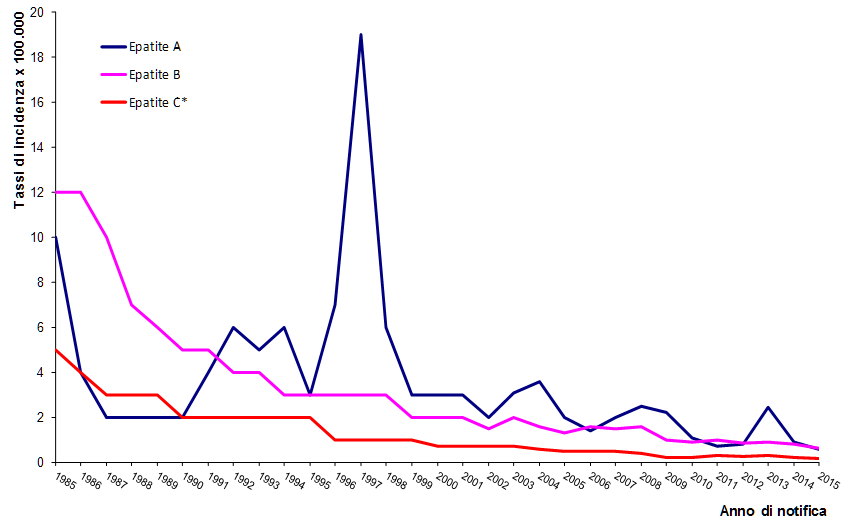
\includegraphics[width=0.3\textwidth]{11/image5.png}
	\end{figure}
  
\subsubsection{Prevenzione}

  Nel tempo vediamo un'iniziale riduzione dell'incidenza che poi si
  mantiene costante. Questo è dovuto all'applicazione di norme generali
  di comportamento che sono le uniche che contengono l'infezione.

  Distinguiamo una prevenzione primaria e una secondaria:

\begin{itemize}
\item
  \textbf{Prevenzione primaria} (evitare infezione): ci concentriamo
  sulle cause di rischio come la promiscuità sessuale, infezioni in
  ambito nosocomiale, trasfusioni e trapianti.

  Si agisce con l' educazione alla salute, con l'educazione alle norme
  di tipo comportamentale (uguali alla HBV) e con le norme di legge:
  regolano le trasfusioni di emoderivati, applicazione di virucidi,
  controllo di unità di sangue , imposizione dal 1989 con ricerca di
  abAntiHCV.
\item
  \textbf{Prevenzione secondaria} (evitare conseguenze): importante
  identificare il soggetto e fare un educazione alla salute e
  eventualmente trattamento con i farmaci innovativi.
\end{itemize}
  
\textbf{\emph{In caso di contatto}}:

\begin{itemize}
\item[1.]
  Detersione accurata, per eliminare ciò che contamina la ferita,
\item[2.]
  Disinfezione,
\item[3.]
  Stesura del rapporto in cui si indica data, durata, tipologia,
  modalità del contatto, conoscenza del paziente fonte, test sierologici
  e virologici.
\item[4.]
  Esami del sangue:
\begin{itemize}
\item
  a tempo zero:enzimi epatici e Ab antiHCV, se negativi:
\item
  dopo 30gg e si aggiuge la ricerca di acidi nucleici, se negativo:
\item
  dopo 60 gg si ripetono le analisi
\end{itemize}
\end{itemize}
  
  Non ci sono evidenze di validità della profilassi passiva.

  Non abbiamo un vaccino a causa della grande variabilità antigentica,
  della tendenza a cronicizzare, dell'impossibilità di replicare il virus
  in vitro, del fatto che l'unico animale su cui si possono fare gli
  studi sono gli scimpanzeè ma sono animali protetti.

  I tipi di possibile vaccino che sono stati studiati sono 2: uno
  impedisce l' infezione (preventivo) e l'altro agisce riducendo rischio
  di cronicizzazione (terapeutico).
